\documentclass[tikz,border=8pt]{standalone}
% Shared look for every TikZ diagram. Load with \input{../../tools/tikz-style.tex}
\usepackage[T1]{fontenc}
\usepackage{lmodern}
\renewcommand{\sfdefault}{lmr}  % diagrams use the same serif as the text
\usetikzlibrary{arrows.meta, positioning, shapes.geometric, calc, fit, backgrounds}
\definecolor{cblue}{HTML}{4C78A8}
\definecolor{corange}{HTML}{F58518}
\definecolor{cgreen}{HTML}{54A24B}
\definecolor{cred}{HTML}{E45756}
\definecolor{cpurple}{HTML}{B279A2}
\definecolor{cgrey}{HTML}{6B6B6B}
\tikzset{
  every picture/.style={font=\sffamily, line width=1.2pt},
  box/.style={draw=#1, fill=#1!12, rounded corners=4pt, align=center, inner sep=7pt, minimum height=1.1cm},
  box/.default=cgrey,
  arrow/.style={-{Stealth[length=3mm]}, draw=cgrey, line width=1.4pt},
  title/.style={font=\sffamily\bfseries\Large},
  note/.style={font=\sffamily\small, text=cgrey, align=center},
}
\AtBeginDocument{\hyphenpenalty=10000 \exhyphenpenalty=10000}

\begin{document}
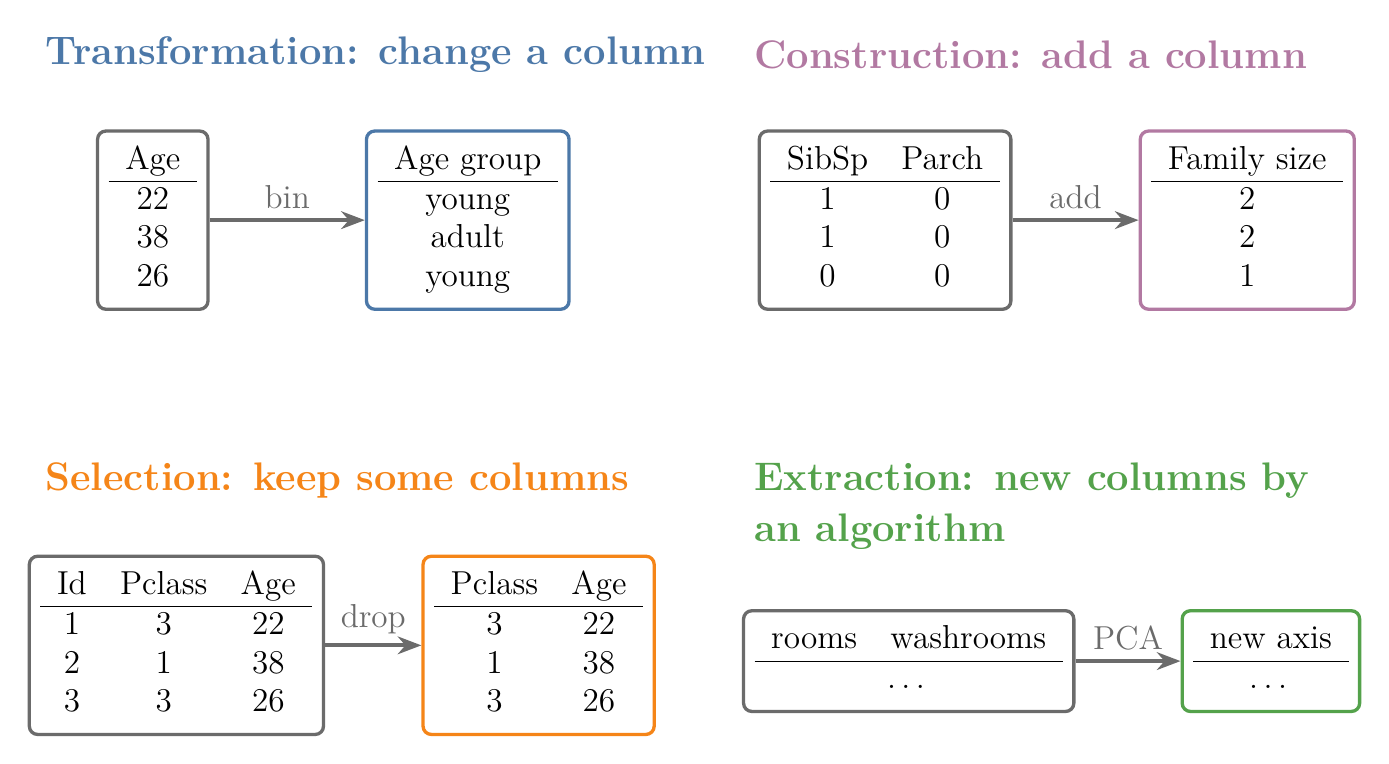
\begin{tikzpicture}[every node/.append style={font=\sffamily\large}]
\tikzset{note/.style={font=\sffamily\large, text=cgrey, align=center}}
  \tikzset{tab/.style={draw=cgrey, fill=white, rounded corners=3pt, inner sep=4pt, font=\sffamily\large},
           hd/.style={font=\sffamily\bfseries\Large, text=#1}}
  % transformation
  \node[hd=cblue, anchor=west] at (-0.2,2.1) {Transformation: change a column};
  \node[tab] (t1) at (1.3,0) {\begin{tabular}{c}Age\\\hline 22\\38\\26\end{tabular}};
  \node[tab, draw=cblue] (t2) at (5.3,0) {\begin{tabular}{c}Age group\\\hline young\\adult\\young\end{tabular}};
  \draw[arrow] (t1) -- node[above, note] {bin} (t2);
  % construction
  \node[hd=cpurple, anchor=west] at (8.8,2.1) {Construction: add a column};
  \node[tab] (c1) at (10.6,0) {\begin{tabular}{cc}SibSp & Parch\\\hline 1 & 0\\1 & 0\\0 & 0\end{tabular}};
  \node[tab, draw=cpurple] (c2) at (15.2,0) {\begin{tabular}{c}Family size\\\hline 2\\2\\1\end{tabular}};
  \draw[arrow] (c1) -- node[above, note] {add} (c2);
  % selection
  \node[hd=corange, anchor=west] at (-0.2,-3.3) {Selection: keep some columns};
  \node[tab] (s1) at (1.6,-5.4) {\begin{tabular}{ccc}Id & Pclass & Age\\\hline 1 & 3 & 22\\2 & 1 & 38\\3 & 3 & 26\end{tabular}};
  \node[tab, draw=corange] (s2) at (6.2,-5.4) {\begin{tabular}{cc}Pclass & Age\\\hline 3 & 22\\1 & 38\\3 & 26\end{tabular}};
  \draw[arrow] (s1) -- node[above, note] {drop} (s2);
  % extraction
  \node[hd=cgreen, anchor=west] at (8.8,-3.3) {Extraction: new columns by};
  \node[hd=cgreen, anchor=west] at (8.8,-3.95) {an algorithm};
  \node[tab] (e1) at (10.9,-5.6) {\begin{tabular}{cc}rooms & washrooms\\\hline\multicolumn{2}{c}{\dots}\end{tabular}};
  \node[tab, draw=cgreen] (e2) at (15.5,-5.6) {\begin{tabular}{c}new axis\\\hline \dots\end{tabular}};
  \draw[arrow] (e1) -- node[above, note] {PCA} (e2);
\end{tikzpicture}
\end{document}
